% COVER PAGE
\begin{titlepage}
\newgeometry{top=3cm, bottom=3cm,
			left=2.25 cm, right=2.25cm}	% Temporarily change margins		
			
% Cover page background 
\AddToShipoutPicture*{\backgroundpic{-4}{56.7}{report/images/auxiliary/Front_Background_Chalmers_GU}}
\addtolength{\voffset}{2cm}

% Cover picture (replace with your own or delete)		
\begin{figure}[H]
\centering
\vspace{1cm}	% Adjust vertical spacing here
%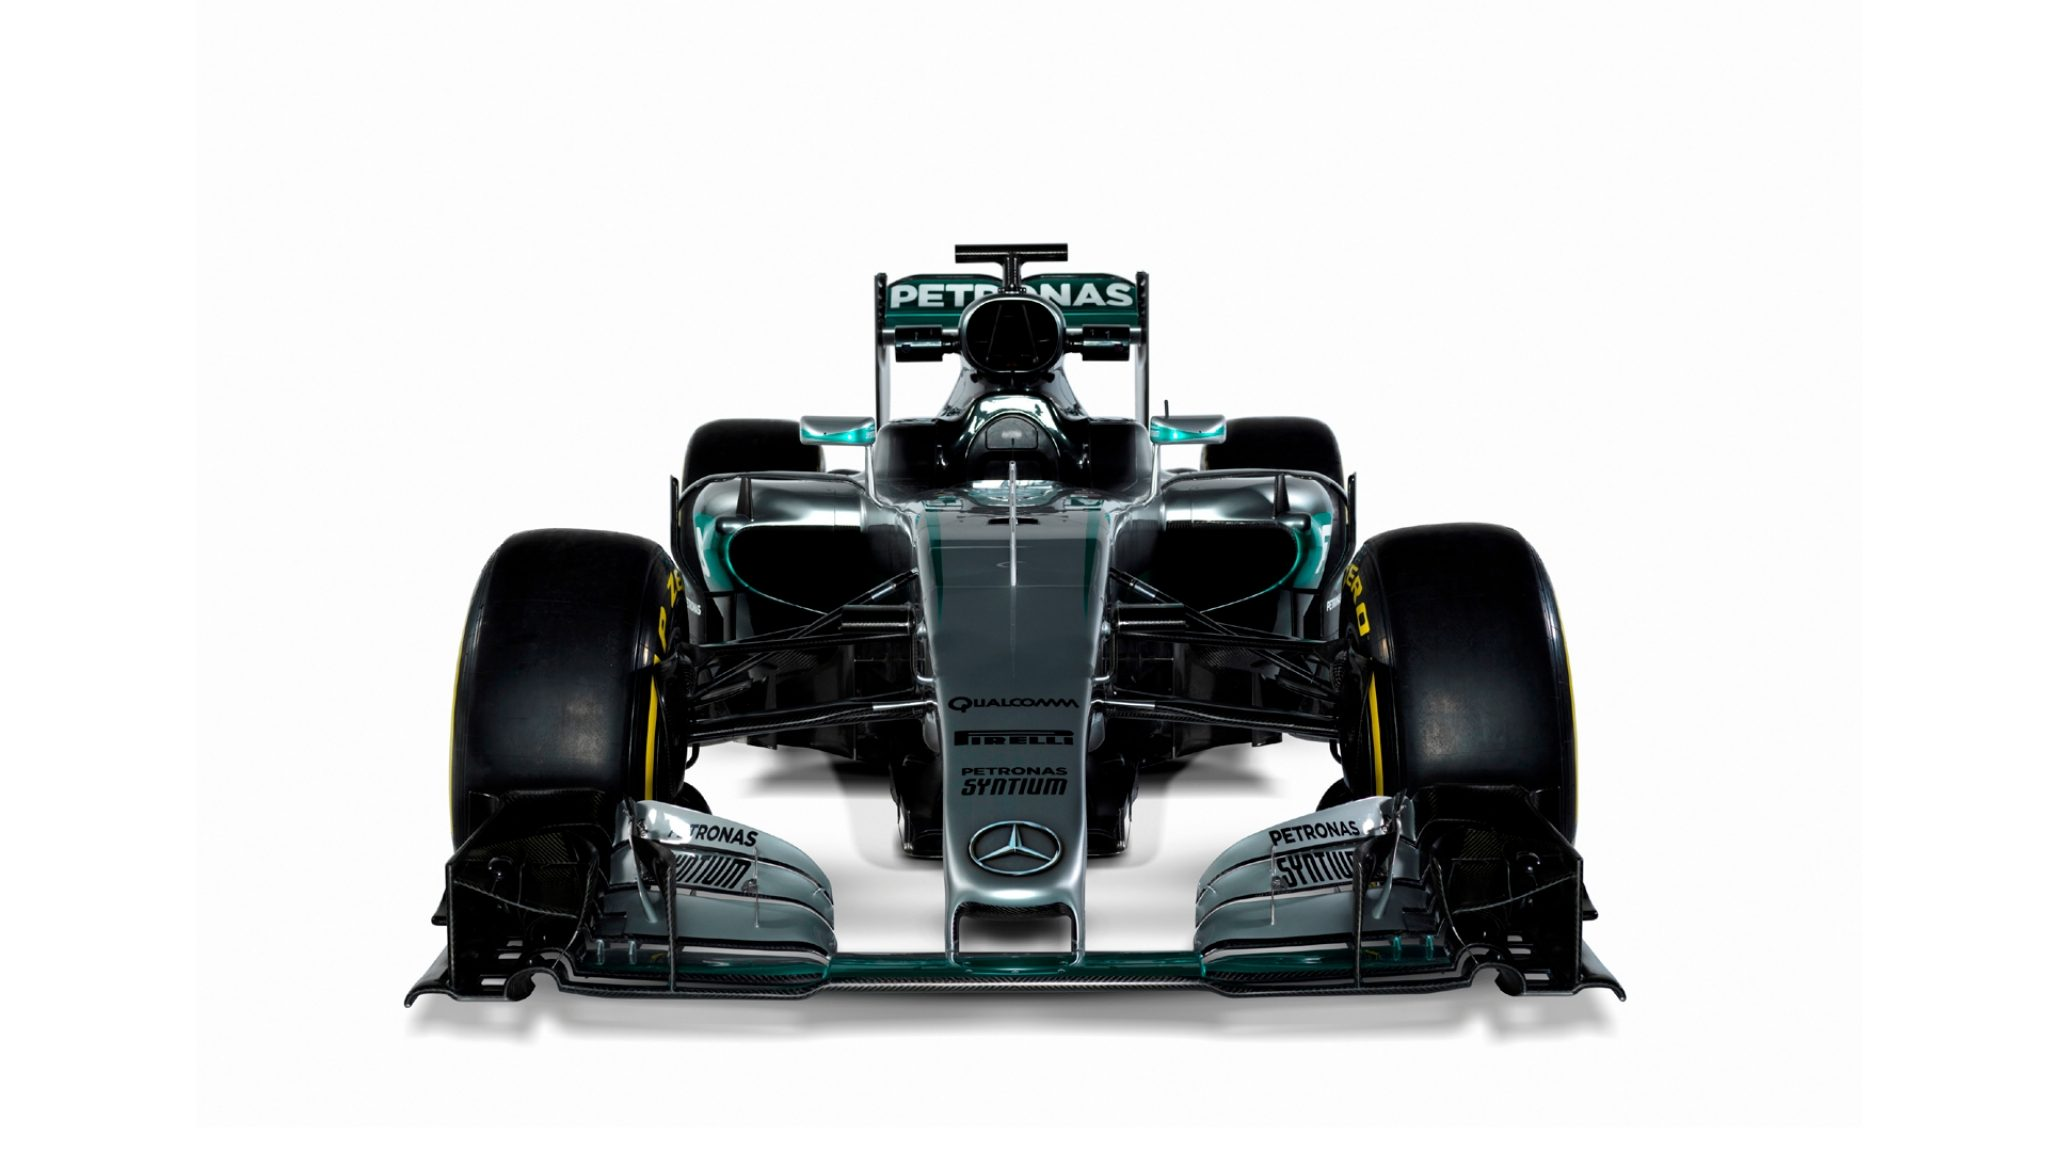
\includegraphics[width=0.9\linewidth]{report/images/logo.jpg}
\end{figure}
\setlength{\parindent}{0ex}
% Cover text
\mbox{}
\vfill
\renewcommand{\familydefault}{\sfdefault} \normalfont % Set cover page font


\textbf{{\Huge Driving Time Trial Laps \\using Neuroevolution}} 	\\[0.5cm]
{\Large The development of a racing AI}\\[0.5cm]
Bachelor's thesis in Software Engineering \setlength{\parskip}{1cm}

{\large Gabriel Alpsten, Daniel Eineving, Martin Nilsson \& Simon Petersson} \setlength{\parskip}{2.9cm}

Chalmers University of Technology\\
University of Gothenburg\\
Department of Computer Science and Engineering\\
Göteborg, Sweden, June 2016\\


\renewcommand{\familydefault}{\rmdefault} \normalfont % Reset standard font
\end{titlepage}


% BACK OF COVER PAGE (BLANK PAGE)
\newpage
\restoregeometry
\thispagestyle{empty}
\mbox{}


% TITLE PAGE
\newpage
\thispagestyle{empty}
\begin{center}
	\textsc{\large Bachelor of Science Thesis }\\[4cm]		% Report number given by department 
	\textbf{\Large Driving Time Trial Laps using Neuroevolution} \\[1cm]
	{\large The development of a racing AI}\\[1cm]
	{\large Gabriel Alpsten}\\
	{\large Daniel Eineving}\\
	{\large Martin Nilsson}\\
	{\large Simon Petersson}
	
	\vfill	
	% Logotype on titlepage	
	%\begin{figure}[H]
	%\centering
	% Remove the following line to remove the titlepage logotype
	%
\includegraphics[width=0.2\pdfpagewidth]{report/images/auxiliary/logo_eng.pdf} \\	
	%\end{figure}	\vspace{5mm}	

    Department of Computer Science and Engineering\\
    CHALMERS UNIVERSITY OF TECHNOLOGY\\
    University of Gothenburg\\
    
    Göteborg, Sweden 2016\\

	%Department of Computer Science and Engineering \\
	%\emph{Division of Software Engineering}\\
	%\textsc{Chalmers University of Technology} \\
	%Gothenburg, Sweden 2016 \\
\end{center}


% IMPRINT PAGE (BACK OF TITLE PAGE)
\newpage
\thispagestyle{plain}
%\vspace*{4.5cm}
\noindent
\textbf{Driving Time Trial Laps using Neuroevolution}\\
The development of a racing AI\\
{\large Gabriel Alpsten}\\
{\large Daniel Eineving}\\
{\large Martin Nilsson}\\
{\large Simon Petersson}\\

\noindent
\copyright ~ Gabriel Alpsten, Daniel Eineving, Martin Nilsson \& Simon Petersson, 2016.\\ \setlength{\parskip}{1cm}
\noindent
Supervisor: K.V.S. Prasad, Department of Computer Science and Engineering\\
Examiner: Niklas Broberg, Department of Computer Science and Engineering \\ \setlength{\parskip}{1cm}

\noindent
Department of Computer Science and Engineering\\
Chalmers University of Technology\\
University of Gothenburg\\
SE-412 96  Göteborg\\
Sweden\\
Telephone: +46 (0)31-772 1000\\
\setlength{\parskip}{0.5cm}

\vfill
% Caption for cover page figure if used, possibly with reference to further information in the report

\noindent
The Author grants to Chalmers University of Technology and University of Gothenburg the non-exclusive right to publish the Work electronically and in a non-commercial purpose make it accessible on the Internet.
The Author warrants that he/she is the author to the Work, and warrants that the Work does not contain text, pictures or other material that violates copyright law.

\noindent
The Author shall, when transferring the rights of the Work to a third party (for example a publisher or a company), acknowledge the third party about this agreement. If the Author has signed a copyright agreement with a third party regarding the Work, the Author warrants hereby that he/she has obtained any necessary permission from this third party to let Chalmers University of Technology and University of Gothenburg  store the Work electronically and make it accessible on the Internet.

\noindent
Department of Computer Science and Engineering\\
Göteborg 2016


%Cover: Temporary image of a car. \setlength{\parskip}{0.5cm}

%Typeset in \LaTeX \\
%Printed by [Name of printing company]\\
%Gothenburg, Sweden 2015

